\noindent Quang học phi tuyến xảy ra khi các chùm sáng có cường độ rất cao, thường là các xung laser ngắn, truyền qua vật liệu. Dưới những điều kiện khắc nghiệt này, vật liệu thậm chí có thể thay đổi bước sóng của ánh sáng. Lý thuyết tổng quát về vấn đề này tương đối phức tạp, nhưng có một số hiện tượng then chốt có thể được lý giải thông qua cơ học lượng tử.

\subsubsection*{Phần A: Khởi động}
\noindent Chúng ta hãy cùng nhau ôn lại một số khái niệm về cơ học lượng tử. Xét một photon có bước sóng $\lambda$ truyền đi trong chân không. Hãy xác định theo $\lambda$ và các hằng số vật lý cơ bản:
\begin{enumerate}
  \item Tần số $f$ của photon.
  \item Năng lượng $E_0$ của photon.
  \item Động lượng $p_0$ của photon.
\end{enumerate}
Bây giờ, xét một chùm laser phát ra các photon có bước sóng $\lambda$. Công suất của laser là $P$.
\begin{enumerate}
  \setcounter{enumi}{3}
  \item Xác định số photon được phát ra trong một đơn vị thời gian.
\end{enumerate}

\subsubsection*{Phần B: Sóng hài bậc hai}
\noindent Bây giờ ta sẽ nghiên cứu quang học phi tuyến. Xét một xung laser có bước sóng trung tâm $\lambda_1$ và tần số trung ứng $f_1$ được chiếu vào một tinh thể phi tuyến. Cường độ laser đủ cao để tinh thể có khả năng hấp thụ đồng thời hai photon, nhưng sau đó chỉ phát ra một photon. Vì đây là một xung, nên nó sẽ chứa một dải các tần số hoặc bước sóng khác nhau.
\begin{enumerate}
  \item Sử dụng định luật bảo toàn năng lượng, hãy xác định tần số trung tâm $f_2$ và bước sóng $\lambda_2$ của photon phát ra.
  \item Giả sử xung laser được phát trong khoảng thời gian $\Delta t$, tìm độ rộng phổ nhỏ nhất $\Delta f_1$ tương ứng của xung. \textit{Gợi ý:} Sử dụng nguyên lí bất định Heisenberg:
        \begin{equation*}
          \Delta t \cdot \Delta E \geq h
        \end{equation*}
  \item Chỉ ra tần số nhỏ nhất $f_1^-$ và tần số lớn nhất $f_1^+$ nằm trong dải phổ.
  \item Vì hai photon có tần số khác nhau có thể được hấp thụ đồng thời và một photon mới có năng lượng bằng với tổng năng lượng của hai photon bị hấp thụ được phát ra nên một xung có tần số lân cận $f_2$ và độ rộng phổ nhất định được tạo ra. Xác định độ rộng phổ $\Delta f_2$ của xung này. Giả sử xung ban đầu chỉ bao gồm các photon có tần số nằm trong khoảng từ $f_1^-$ đến $f_1^+$.
  \item Tìm thời gian phát của xung mới. Bình luận về kết quả mà bạn tìm được.
\end{enumerate}

\subsubsection*{Phần C: Bảo toàn động lượng}
\noindent Cho đến hiện tại, ta chỉ mới xét đến định luật bảo toàn năng lượng. Tuy nhiên, động lượng vẫn phải được bảo toàn. Để làm được điều đó, cần phải xét đến chiết suất của môi trường. Nhìn chung, chiết suất phụ thuộc vào bước sóng (mối quan hệ này được gọi là hiện tượng tán sắc). Giả sử chiết suất của tinh thể đối với xung laser ban đầu là $n_1(\lambda_1)$ (không đổi trong toàn bộ độ rộng phổ $\Delta f_1$) và chiết suất của tinh thể đối với xung mới là $n_2(\lambda_2)$. Trong toàn bộ phần này, giả sử xung tới có phương vuông góc với bề mặt của tinh thể, do đó theo định luật Snell, xung sẽ tiếp tục truyền vuông góc vào trong tinh thể.
\begin{enumerate}
  \item Giải thích tại sao chiết suất lại quan trọng đối với định luật bảo toàn động lượng.
  \item Xác định mối quan hệ giữa $n_1$ và $n_2$ để động lượng của photon được bảo toàn.
  \item Hãy khảo sát điều gì sẽ xảy ra nếu điều kiện trên không được thỏa mãn. Trong Hình 2, sóng ban đầu (có tần số $f_1$) khi vừa đi vào tinh thể được biểu diễn cùng với sóng mới (có tần số $f_2$).
        \begin{figure}[H]
          \centering
          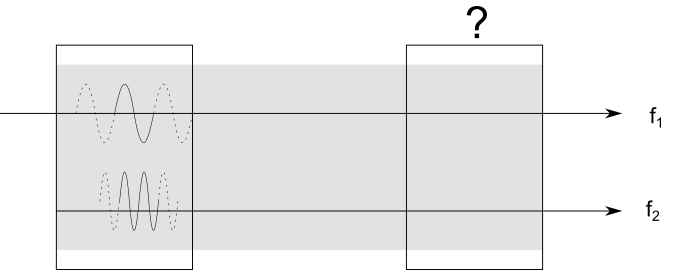
\includegraphics[width=0.5\textwidth]{Figures/Problems/Fig 2.1.png}
          \begin{center}
            \figurename{ 2}
          \end{center}
        \end{figure}
        \vspace{-0.5cm}
        Hãy hoàn thiện hình vẽ ở đầu ra của tinh thể bằng cách vẽ hai sóng trong trường hợp điều kiện bảo toàn động lượng bạn vừa tìm ra ở trên không được thỏa mãn. Giải thích hình vẽ của bạn bằng các lập luận và phương trình.
  \item Nếu điều kiện bảo toàn động lượng không được thỏa mãn thì độ dày của tinh thể sẽ ảnh hưởng như thế nào đến cường độ của xung có bước sóng $\lambda_2$ phát ra khỏi tinh thể?
\end{enumerate}
